% !TEX root = _main.tex 
% ==========================================
% ここから本文．あとは各自で
% ==========================================

%1
\section{はじめに}
音楽は，今日多くの人にとって日常の一部となっており，様々な空間において音楽を楽しんでいる．その楽しみ方も，聴く，歌う，踊る，見るなど多岐にわたり，音楽は人々が交流し，思いを共有したりする手段の1つとなっている．

しかし，コロナ禍によって，音楽の楽しみ方が制限され，実際にライブ会場やカラオケボックスに行くことが難しくなり，音楽がある空間（以下音空間とする）における雰囲気というもの肌で感じるということもできなくなってしまった．また，それに伴い音楽を通した人々の交流もSNS上や，画面越しのリモートとなってしまい，音楽活動そのものが限られたものになってしまった．しかし，このことでリモートやVR等の電子技術が大きく進歩するきっかけとなった一方で，多くの音楽活動が対面での活動へと戻ってきた．これは，人々が音空間において雰囲気を肌で感じ，その興奮や感動を共有し交流することが，重要な要素であるからではないかと考える．

コロナ禍での電子技術の進歩は，音楽の見せ方も大きく変えた．音空間における映像や特殊効果などの視覚表現の進歩は，人々の音楽の楽しみ方の可能性を広げている．その一方で，これらの視覚表現を身近に扱うにあたっては専門的知識や技術，道具などが必要になるため，再現することは容易ではない．

そこで，本研究では，容易な技術や素材を用いて，音空間に対して視覚表現を付与する音映像空間を作品制作を通して表現することを目的とする．作品を制作するにあたって，重要視する点は音楽の要素を多角的にとらえ，その魅力を音空間として表現することとする．その条件として，空間の雰囲気に入り込んでもらい，その場での人々の交流に重きを置くために，身近な空間での生演奏を音空間とする．それに対し，演奏者，聴衆，演出の様々な立場において，作品全体を考え，自身が音楽から感じる心象を視覚化し伝えることも重要視する．




\section{演出表現における音楽要素}

音楽は様々な要素から成り立っており，これらは演出表現を行う際に大きな役割を持つ．この音楽の要素は演出表現において，大きく「譜面的要素」と「背景的要素」の２つに分けることができる．これらの要素は演出表現を行う際にも重要な要素となる．本制作においてもこれらの要素を意識して作品制作を行う．
\subsection{音楽の譜面的要素}
はじめに，音楽の「譜面的要素」とは，音高や音量の変化，コード進行による曲調の変化，楽器構成などである．「譜面的要素」は聴衆にとって感情や認知などに影響をもたらすことが多い．

これについてまず，私が注目したのは音楽プロデューサーの田中隼人のクリスマスソングらしさについての実演解説の記事だ\cite{xmassong}．ここで田中氏は音楽と感情はリンクしたものであり，メロディや曲調などはカテゴライズしやすいがクリスマスっぽいという感情はないため，共通した楽曲のイメージはないと語っている．しかし，その中でクリスマスらしさを感じる要因として，人々の習慣や経験に紐づいた文化的背景や共有前提が存在すると考えられている．例えば，スクイズベルという楽器はほぼクリスマスにしか使われない楽器であり，巷でクリスマスソングといわれるものには使用されている，と記事に記載されている．また多くのクリスマスソングはほぼすべてが“C”のコード、ハ長調から始まり，その理由を田中氏はキーの中で一番明るいのはCコードであり，クリスマスといったポジティブなイベントとの関連性を指摘している．このように共通した楽曲のイメージが存在せずとも，楽器やコード進行による共有前提が，抽象的なイメージの情景想起の手助けになっていることが分かる．

さらに，2014年広島大学の森らの論文では，音楽によってもたらされる特異的な感情反応などについて示されている\cite{Mori14}．例えば日常生活における混合感情も音楽構造の組み合わせによって生じる可能性が示されている．ここでの組み合わせでは，速いテンポで長調の曲と歌詞の組み合わせによる，喜びと悲しみの混合感情や音楽特融の悲しい音楽による快感情などに対する研究が挙げられている．さらに，音楽による感情の時系列評価や生理反応についても示されており，音楽によって心理に対する影響のみではなく，身体的レベルでの影響についても述べられている．このような音楽が心身に及ぼす影響は，荒川らの研究のように医療や福祉における人のリラクゼーションや感情、知覚、認知を活性化などに使用されている例は多数ある\cite{Arakawa96}．

これらのことに注目し，演出表現において神野らは歌詞や曲調を手掛かりとした照明演出システムを実現させている\cite{Kanno22}．

\subsection{音楽の背景的要素}
次に音楽の「背景的要素」とは，曲の制作過程や，演奏者の表現，楽曲が何かの主題歌であるかどうかなどの情報などが例として挙げられる．「譜面的要素」は不変なものであるが，この「背景的要素」の受け取り方は各個人によって大きく変わる．まずそもそも，楽曲についての情報や演奏者などの情報などについて知らなければ，その楽曲における「背景的要素」はないも同然になる．しかし一方で「背景的要素」には聴衆が情景音楽から情景を想起させるための手掛かりとなる具体的な情報を持っていることが多いことが多い．例えば，楽曲が何らかの主題化となっている場合，そのアニメ等のイメージがそのまま楽曲のイメージとして情景の想起につながる．また，作曲者や歌手，演奏者の背景知識がある場合，それらの影響を大きく受けることもあるだろう．

\subsection{本研究における音楽的要素の表現}
これらのように音楽はその要素ごとに人々に様々な影響をもたらしており，演出表現においても重要な要素になっている．本作品ではこれらの要素踏まえ，音楽の持つ世界観を魅せることを目標とした表現をおこなう．そのための条件として全ての作品において福知山公立大学3201の教室を利用して，生演奏による音楽映像空間の作品制作を複数行うこととする．

本作品において音楽的要素から生み出される世界観を魅せるために主に３つのことを意識した作品制作を行う．

まず1つ目は生演奏を行う楽器が持つ世界観を活かすことだ．同じ楽曲であっても，演奏する楽器によっては楽曲から受け取る印象も大きく変わる．そのため，各作品で使用する楽曲に対して魅力を引き出すことのできる楽器，または楽器の魅力を引き出すことのできる楽曲を使用し，演出において楽器の生演奏が生み出す世界観を表現することを意識する．2つ目は楽曲そのものが持つ世界観を再現し魅せることである．その楽曲が使用されている場面や作品等の背景的要素を視覚化し再現することで，楽曲の世界観を表現する．3つ目は音空間において演奏者を魅せるということである．演奏者を単なる音源として扱うのではなく，演奏者も音楽の要素の1つとして扱い，作品の世界観に溶け込ませる，または作品において演奏者を魅せるということを意識する．

以上のような点を意識して作品制作を行った．




\section{作品の世界観を再現する演出表現}
\subsection{作品制作の背景}
第1回目の作品制作の題材に選んだ楽曲はアラジンの主題歌である「A Whole New World」\cite{Aladdin}という楽曲である．この曲は自身がゼミの活動としてピアノ演奏の練習をしていた曲であり，ゼミ内で発表する機会があったため，自身の演奏に合わせた演出を行うことを目標として，作品制作に取り組んだ．本作品においては，複数人のグループでの制作とした．筆者は自身が演奏者となりながら，総合的な演出の構想や，メンバーへの指示，演出制作などを行った．


\subsection{A Whole New Worldの世界観}
この「A Whole New World」という楽曲を聴くとやはり，多くの人がディズニー映画のアラジンを想起するだろう．アラジンは、貧しい青年アラジンが偶然手に入れた魔法のランプを使い、願いを叶える力を持つジーニーと出会う物語である。アラジンは王女ジャスミンに恋をし、彼女に近づくために「王子になる」という願いを叶えてもらう。しかし、悪い魔法使いジャファーがランプを奪おうと企み、アラジンはジーニーや友人たちと協力してジャファーを倒す。最終的に、アラジンは自分の勇気と誠実さを示し、ジャスミンとの愛を勝ち取るという物語となっている。

この「A Whole New World」という楽曲は作品内で，アラジンがジャスミンを魔法の絨毯を使って，世界をめぐる冒険に誘う場面で流れる楽曲となっている．曲名の「A Whole New World」を日本語に直訳すると，「全く新しい世界」という意味になり，その曲名の通り，2人は夜空を飛びながら，自由や新しい世界の美しさを歌で共有する．このシーンは，幻想的な景色と感動的なデュエットが特徴，アラジンの映画を象徴するロマンチックな場面となっている．


\subsection{舞台構成}
使用する3201教室における機材の配置図を\figref{fig:aladdin-system}に示す．
3201教室に備え付けてある，スクリーンと吊り下げ型のプロジェクターを軸とした配置設定を考えた．スクリーンの後ろに，演出で使用するドライアイスを配置し，スクリーン周辺とピアノの装飾としてライトを複数配置する．操作用のPCはスイッチャーにつないで，演奏に合わせてリアルタイムで操作し，天井プロジェクターへと接続する．


\begin{figure}[tb]
	\centering
	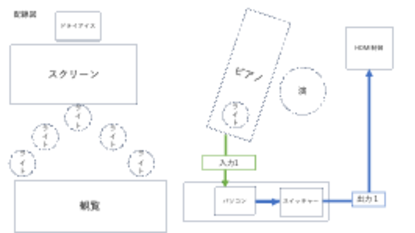
\includegraphics[width=\hsize]{fig/fig1-aladdin.pdf}
	\caption{アラジンにおける機材の配置}
	\label{fig:aladdin-system}
\end{figure}


\subsection{演出のねらい}
「A Whole New World」のピアノ演奏に合わせた演出として，映画「アラジン」における象徴的なアイテムとしてでてくる魔法のランプと魔法の絨毯に注目して，アラジンの世界観を表現することを意識した作品制作を行うことにした．


\begin{figure*}[tb]
	\centering
	\begin{minipage}
		{0.4\hsize}
		\centering
		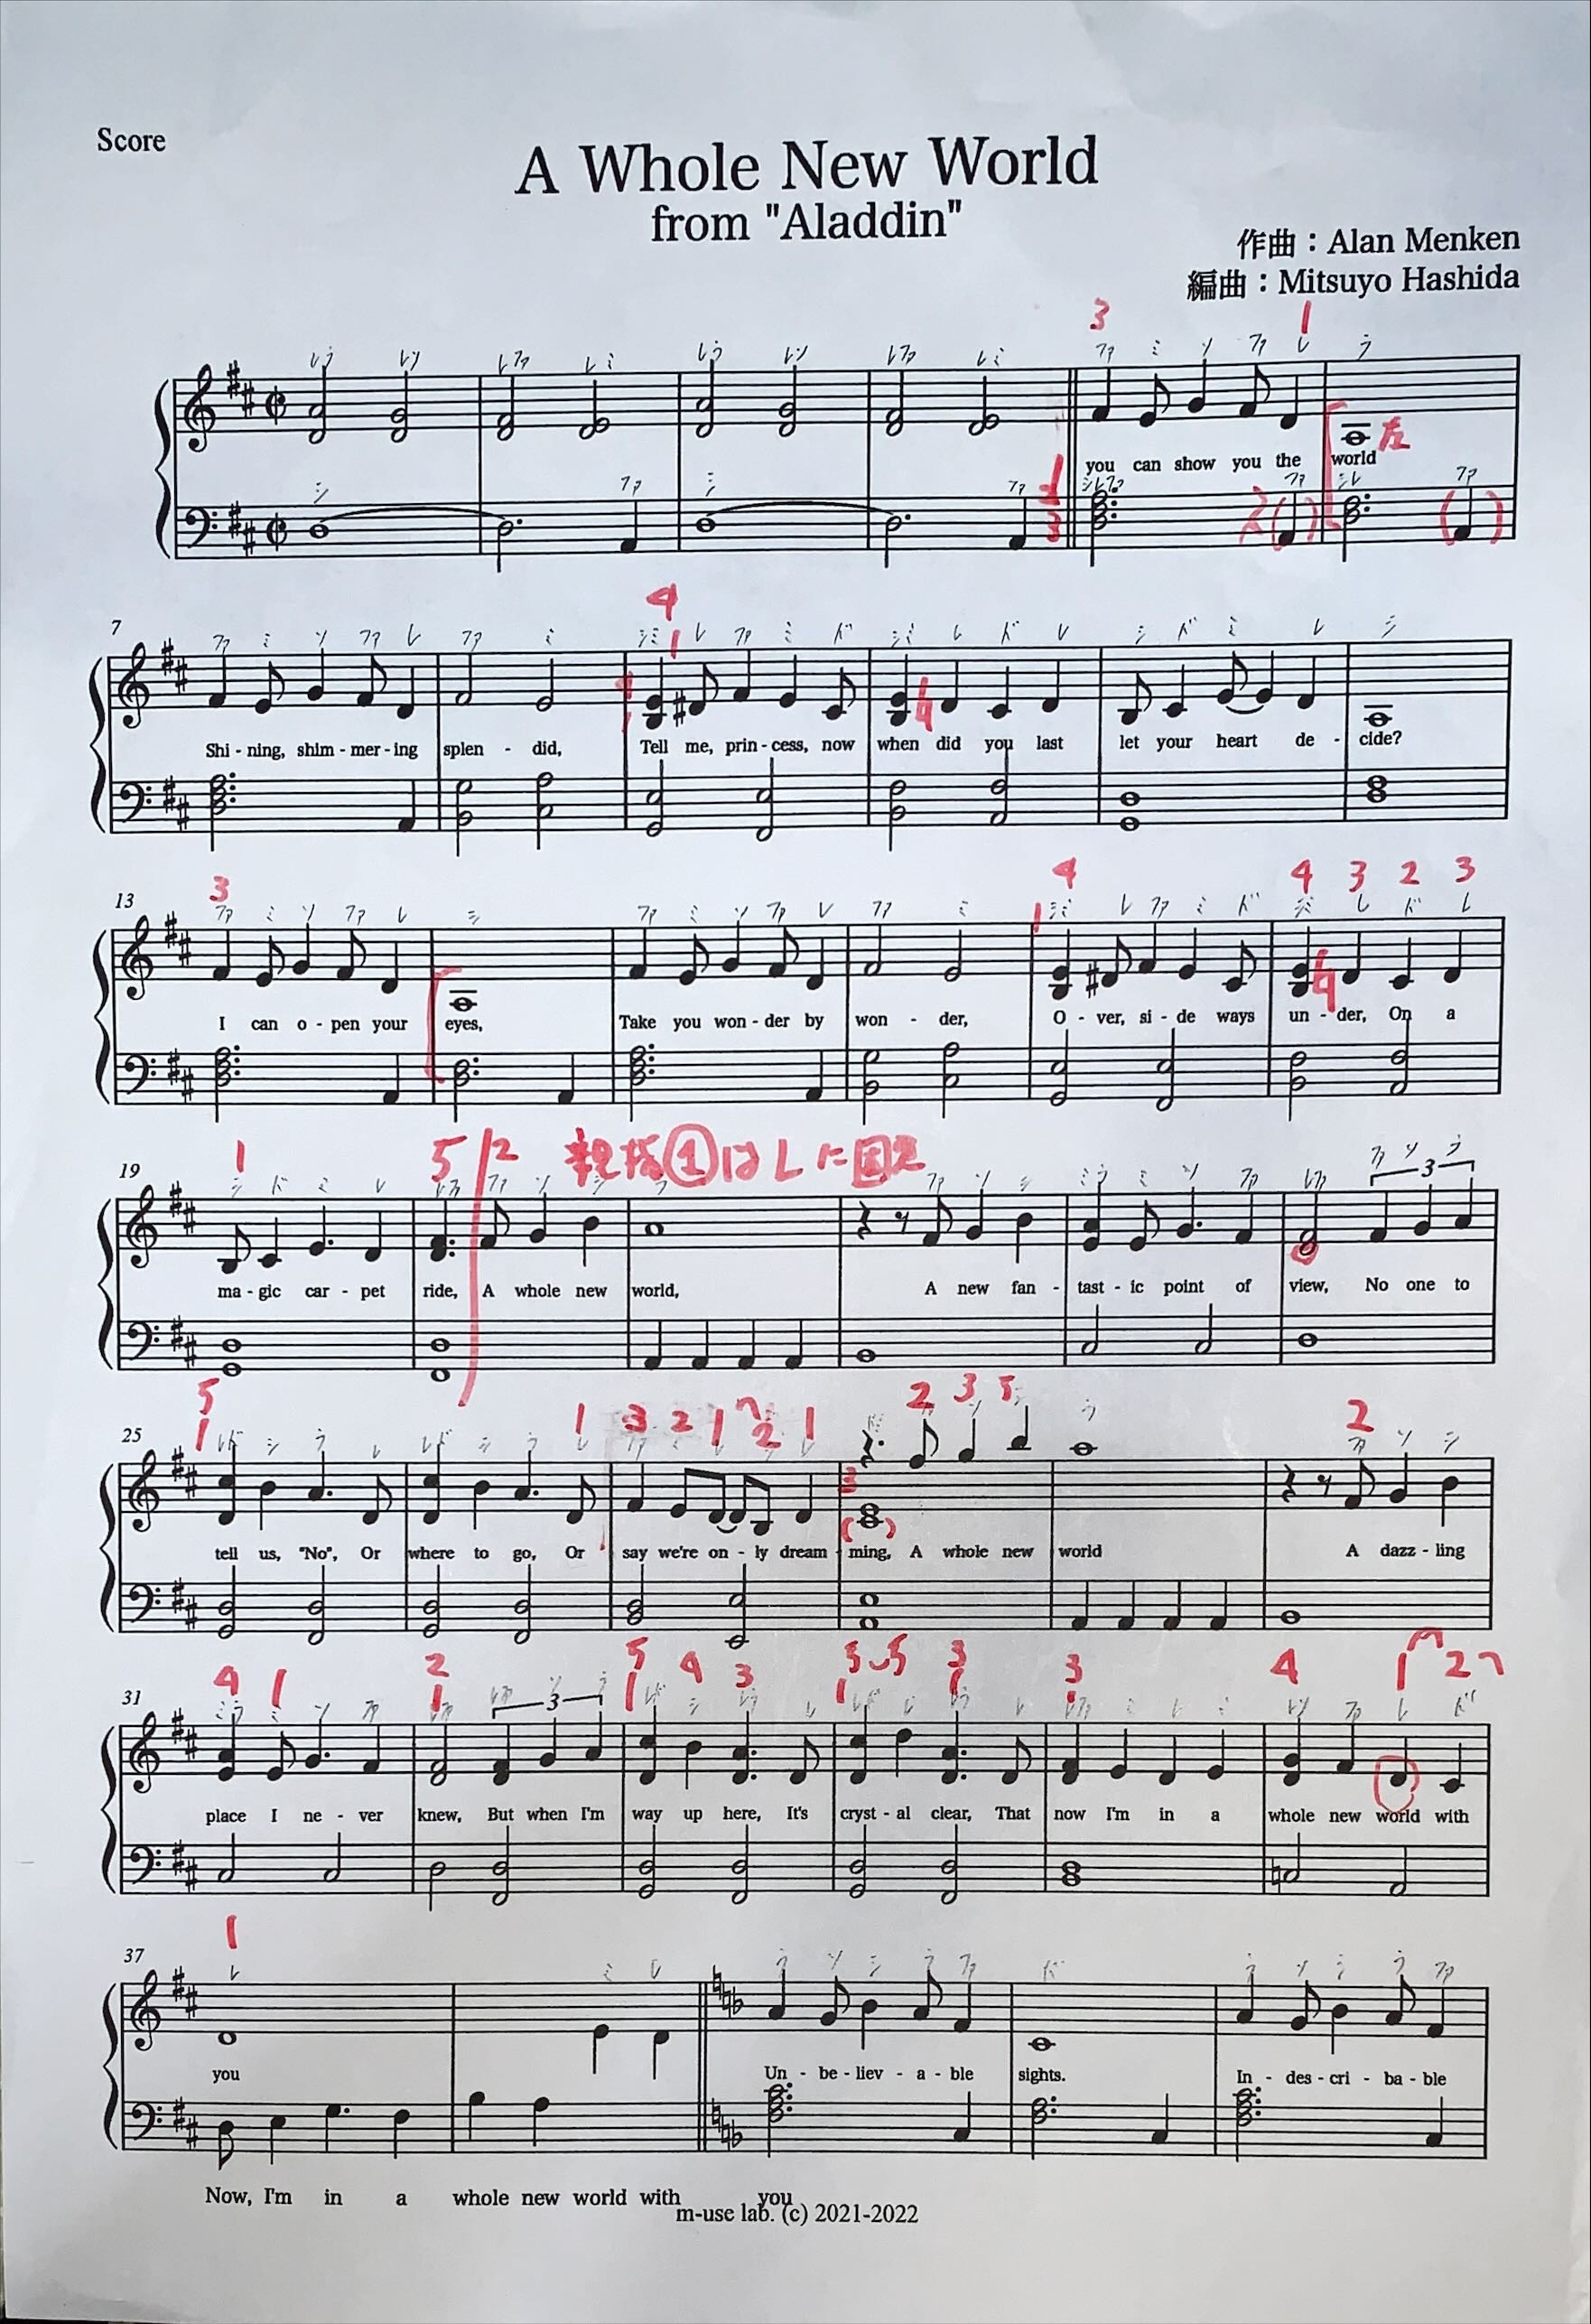
\includegraphics[width=\columnwidth]{fig/IMG_0563.JPG}
	\end{minipage}
	\begin{minipage}
		{0.4\hsize}
		\centering
		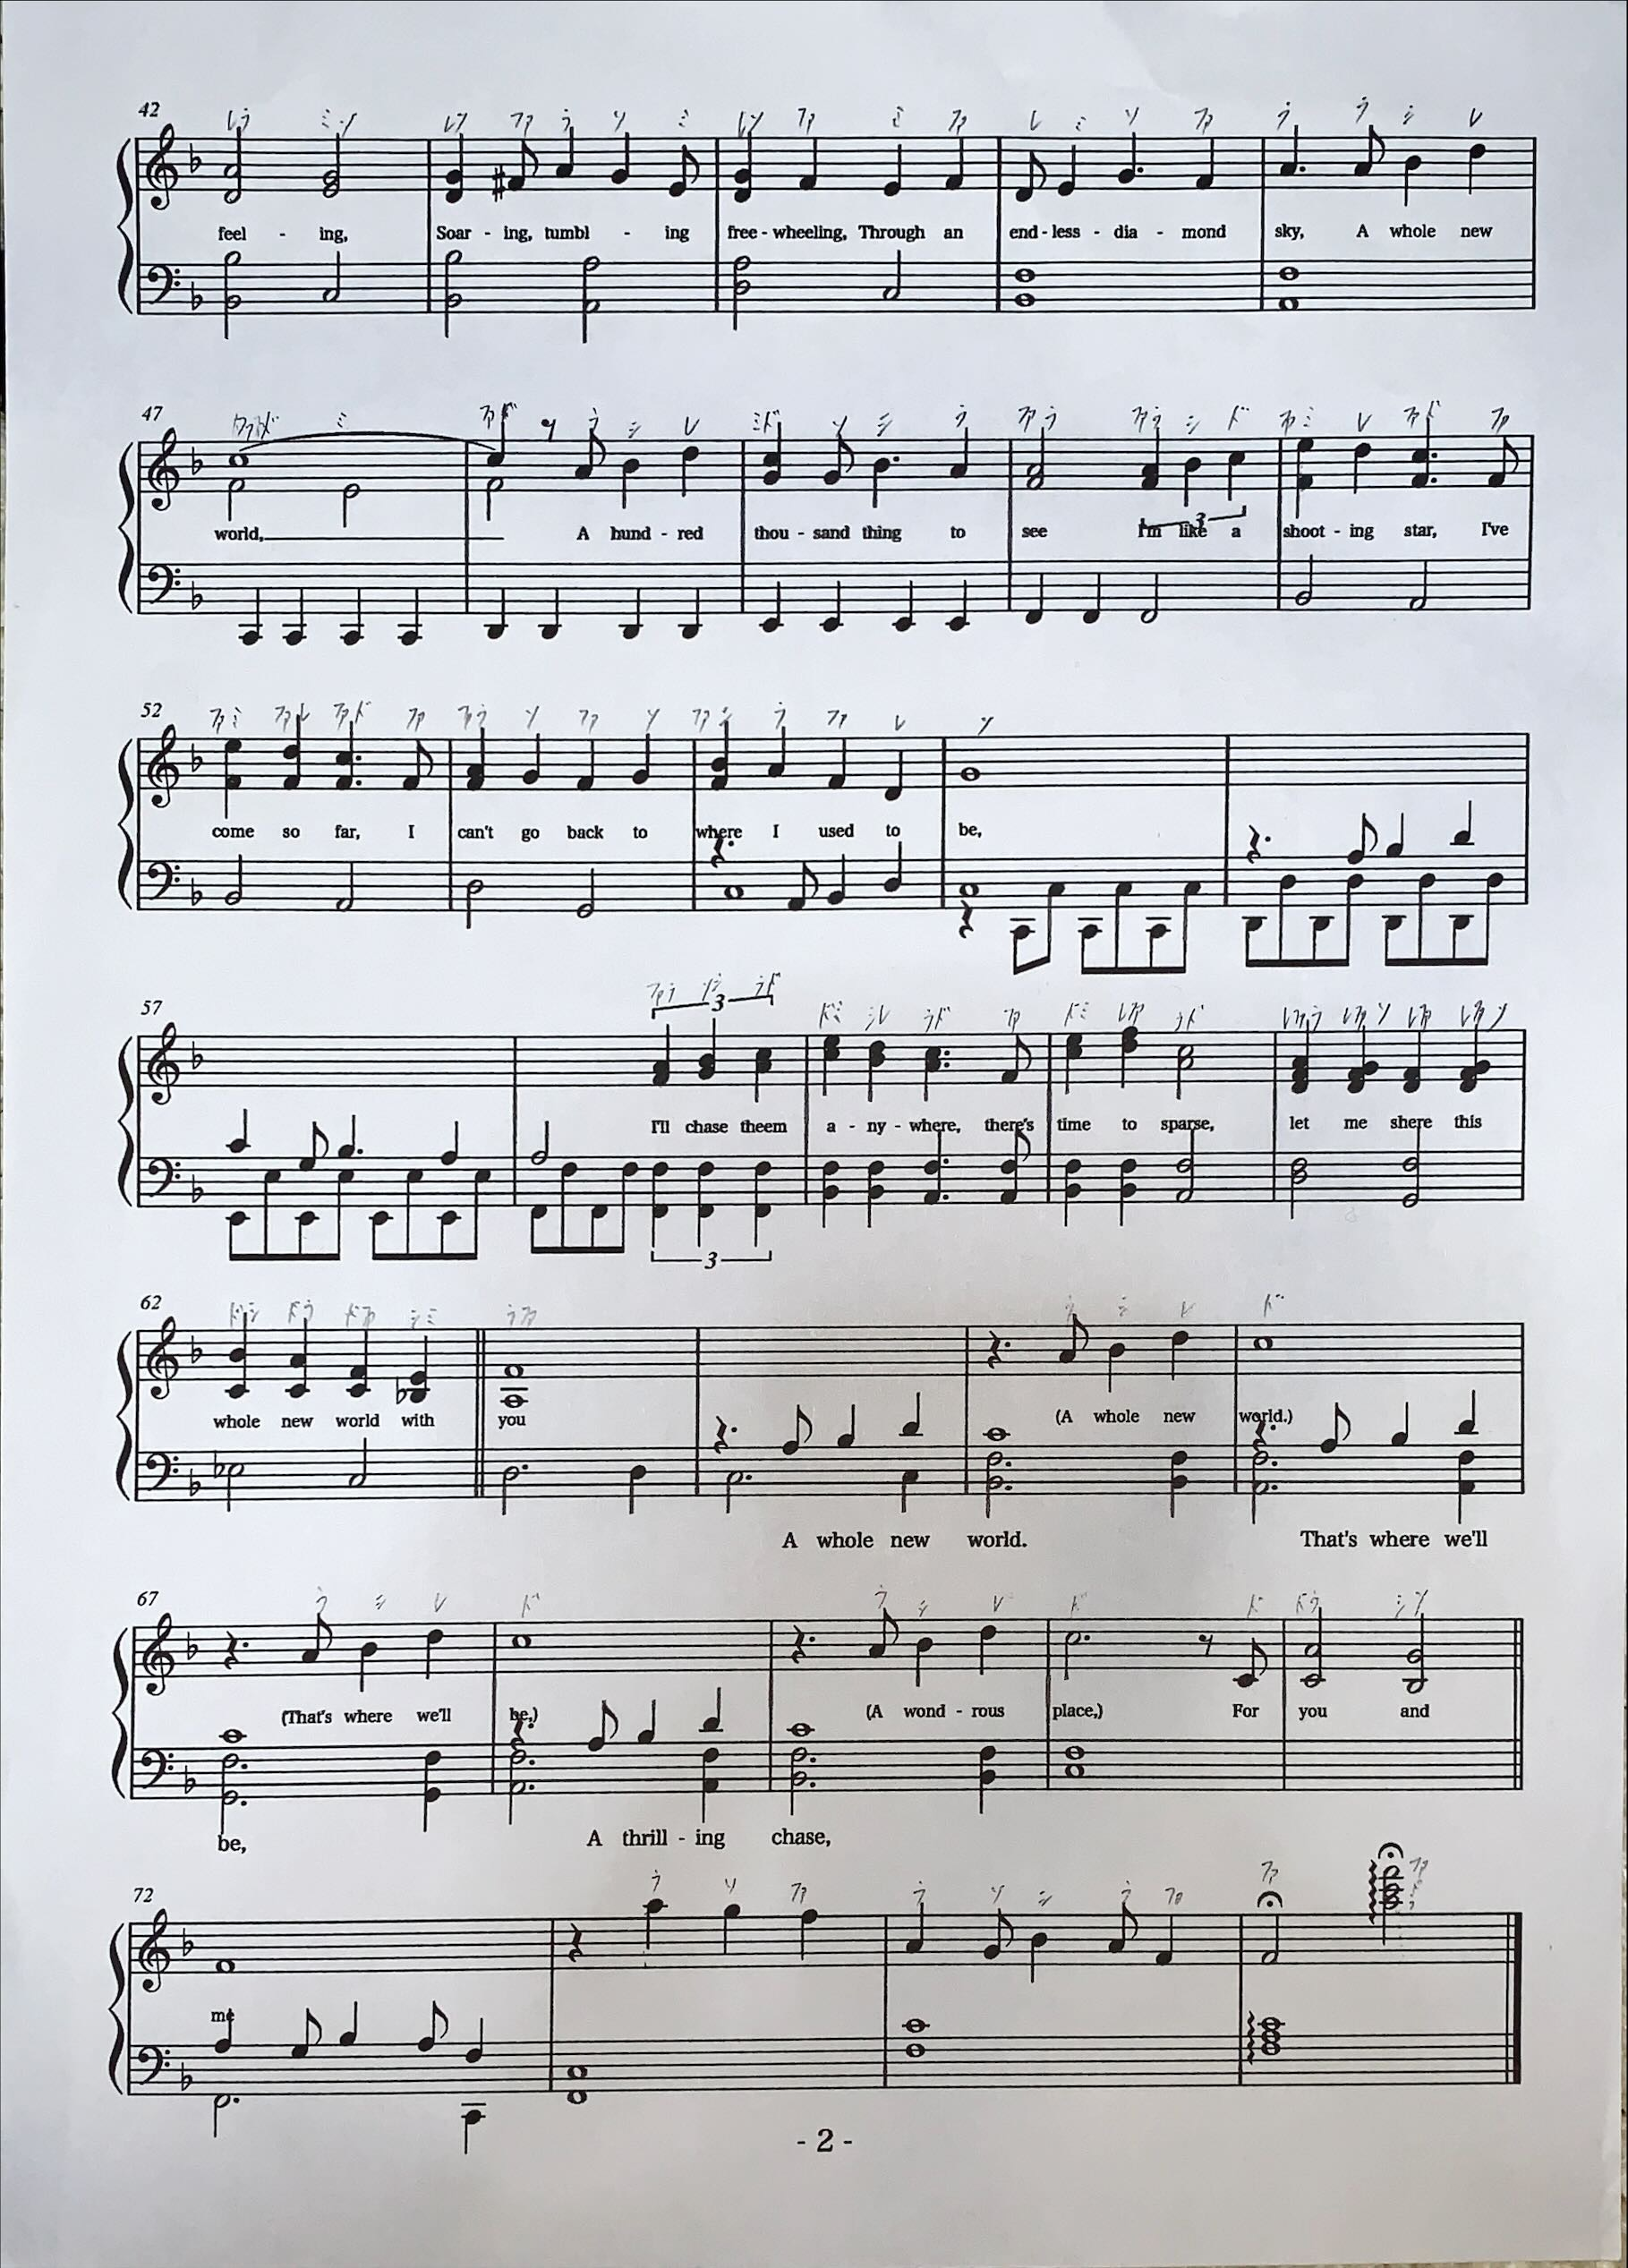
\includegraphics[width=\columnwidth]{fig/IMG_0564.JPG}
	\end{minipage}
	\caption{使用した「A Whole New World」の楽譜}
	\label{fig:aladdin}
\end{figure*}

\subsubsection{映画「アラジン」との音楽表現の異同}
アラジンの映画内での「A Whole New World」では，管楽器をはじめとして，グロッケンや鈴といった高音かつ装飾系の打楽器など，様々な楽器の組み合わせによって幻想的な夜空の旅を表現している．今回は，ピアノの生演奏での演出表現とすることで，音楽の魅力をシンプルかつ滑らかに表現することができる．特にメロディラインの美しさや，楽器1つで男性のアラジンと女性のジャスミンなど多様な表現が可能である点がピアノ演奏での特徴である．

また，映画内の楽曲ではアラジンとジャスミンの会話の後，魔法の絨毯に乗って2人が歌唱を始めるため，イントロらしいものがないまま楽曲が始まる．一方で，CDなどに衆力されているものについては短いイントロがついている．今回ピアノ演奏が初心者である，筆者が演奏をするということもあり，楽譜における４小節目まで独自のイントロをつけた．さらに，ピアノ演奏が始まる前と演奏終了後に，チームのメンバーが独自に作曲し，編曲した音を流し，それぞれ導入部分と結びの部分とした．



\subsubsection{アラジンの世界を再現する映像空間表現}
まず，演奏の前の導入に合わせて魔法のランプから靄が出てくる様子を投影し，同時にドライアイスによっても現実空間でも靄を実際に出すことで，靄に包まれてアラジンの世界へと入り込んでいく様子を表現した．ピアノ演奏が始まると，魔法の絨毯で雲の中を飛んでいる様子を映像投影し，2番に入ると流れ星がMIDIの出力によってピアノ演奏に合わせて流れる映像となっている．また，ラスサビに向けては雲の中を抜けて，星が月が雲の隙間から見えてくるような，雲の上に向けて飛んでいるような様子を表現した．最後は，結びの音源と同時に靄が魔法のランプに戻っていくことで，アラジンの世界から，現実の世界へと戻っていく様子を再現した．

\begin{figure*}[tb]
	\centering
	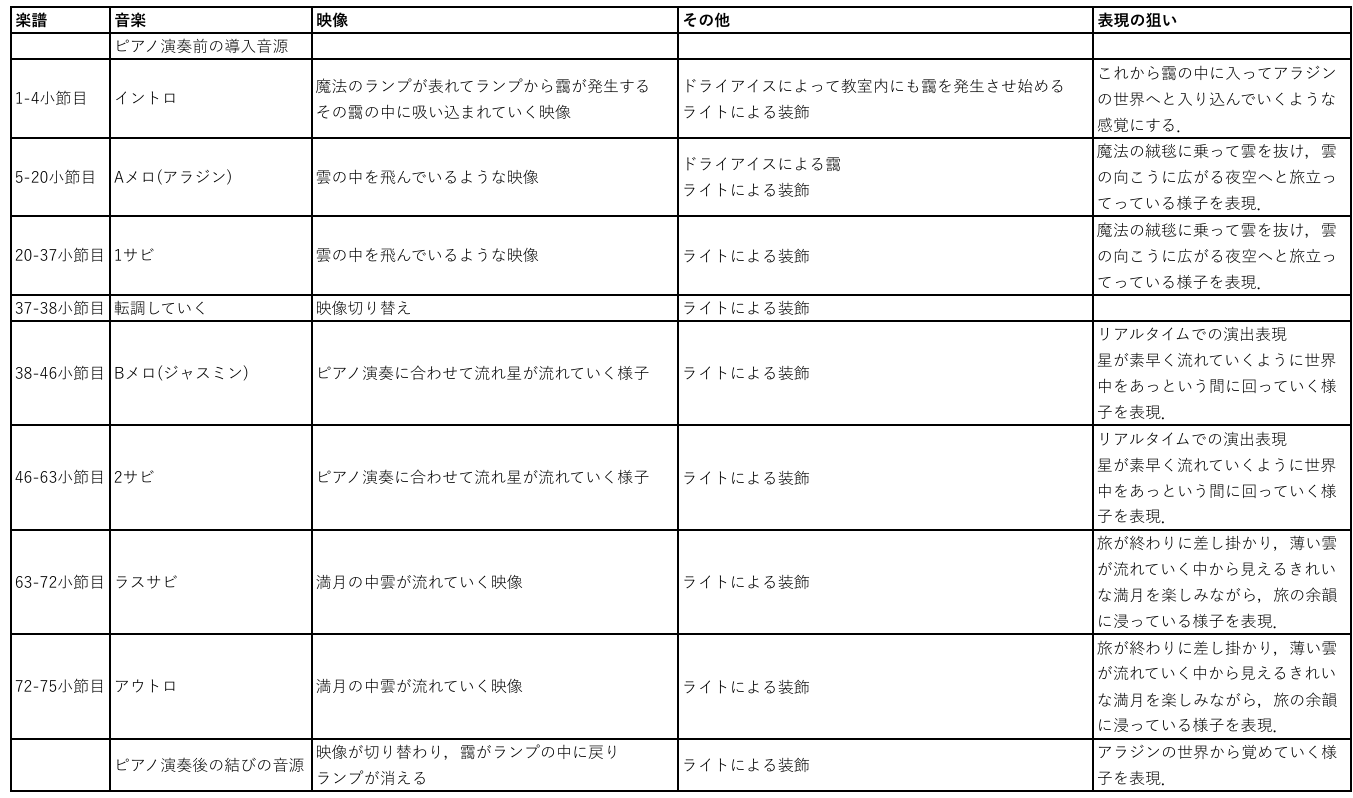
\includegraphics[width=\hsize]{fig/aladdin.png}
	\caption{「A Whole New World」の演出シナリオ}
	\label{fig:aladdin-scenario}
\end{figure*}


\subsection{作品発表と振り返り}
\subsubsection{作品発表}
本作品をゼミ内での演奏会で橋田ゼミのメンバー15名程度に対して発表を行った．

\begin{figure}[tb]
	\centering
	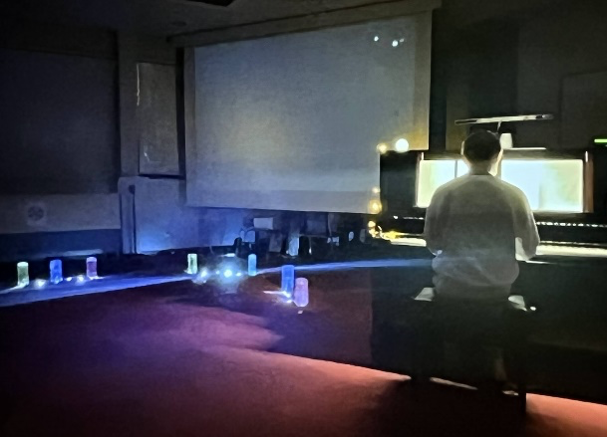
\includegraphics[width=\hsize]{fig/fig2-aladdin-play.png}
	\caption{「A Whole New World」の作品発表}
	\label{fig:aladdin-play}
\end{figure}

\subsubsection{振り返り}
本作品では，初めての作品制作として，ピアノ初心者である，筆者の演奏に合わせて1曲最初から最後まで何かしらの演出をとにかく組み込むことを目標とした．その中で本作品において最も意識・工夫した点は，アラジンの世界観を再現することであった．そのために映像のみではなく，現実空間でもアラジンの世界観を表現した．例えば雲や靄を表現するために，ドライアイスを用いた演出を行ったり，月や星の光を表現するためにライトの配置を行ったりした．また，筆者がピアノ初心者ということもあり，演奏者に演奏の自由度を与えるために，星の流れる様子をピアノからMIDIの出力による制御とすることで演奏速度やテンポにとらわれない演出を行うことができた．また映像の切り替えを手動で行うことで，ミスやテンポに左右されない映像表現ができた．

一方でドライアイスによる効果はそれほど大きくなかったため，今後何らかの対応が必要となってくる．また映像の中身についても今回はフリー素材等を多く使用してしまったため，まだまだアラジンの世界観を表現するための映像としては表現に幅がなく，演奏者の自由度のために映像の切り替えもすべて手動で行ったためストーリーの表現の幅がかなり狭くなってしまった．

また，映像が備え付けのスクリーンのみでの投影で教室を空間として生かせていなかったため，今後は演奏者を活かしつつ映像投影の幅を広げることを目標とする．映像の中身も，自身で1から作りより，楽曲の世界観に入り込めるようなストーリー性を持たせたような映像作品にする．


\section{映像空間の拡張を目指した演出表現}
\subsection{作品制作の背景}
アラジンの「A Whole New World」の作品制作の振り返りをもとに，次の作品制作に取り組んだ．第2回目の作品の曲に選んだものは，大塚愛の「プラネタリウム」という曲である\cite{Planetarium}．この曲を選んだ理由としては，作品の発表の時期が夏終わりであり，個人的にも好きな曲であるため，生演奏で披露する際には，その空間と雰囲気もうまく利用できるのではないかと考えたからである．

\subsection{プラネタリウムの世界観}
\subsubsection{楽曲制作の由来}
この「プラネタリウム」という楽曲について，歌い手であり，作詞作曲も手掛けた大塚愛がインタビューで楽曲の制作について語っている\cite{interview}．この楽曲について，それまで作者が出してきたバラードのようにラブソングではなく，中世的なナンバーになっていると語っている．また，元気にはしゃいでいるようなサマーソングではなく夏の終わりを感じさせるような時期の曲になっているとも述べている．さらにこの楽曲のタイトルである」プラネタリウムについて，作者がプラネタリウムを見た際に，実際に見る平面的な星空ではなく，くるくると早送りで見るプラネタリウムの映像が印象的に残り，タイトルをつけたと語っている．

\subsubsection{筆者が感じた楽曲の世界観}
この曲について私は，切なくも美しいバラード曲で，好きな人とのこれまで記憶と叶わない願いと別れの切ない様子を表現していると考える．この曲は、ゆったりとしたメロディにのせて，夏の夜空や星，はかなく散っていく花火のなどの目まぐるしく変化する，夏の切ない夜の情景を想起するような楽曲になっていると感じた．そこで，その切ない様子を表現するために使用する楽器をピアノのみとすることにし，その音に合うような映像表現を行うことにした．

\subsection{舞台構成}
使用する3201教室における機材の配置図を\figref{fig:planet-system}に示す．今回も前回と同様3201教室に備え付けてある，スクリーンと吊り下げ型のプロジェクターを軸とした配置設定を考えた．そのスクリーンに合わせて，ピアノを隣に配置し，そのピアノの側面にも映像を投影するために，正面にプロジェクターを用意し，操作用のPCを配置した．ピアノは直接プロジェクターで投影してしまうと，反射して映像が見えないことがあるので，黒い布をかぶせて対応した．また，ピアノ演奏者に対して3台のカメラを設置することで，演出の一部に組み込んだ．今回カメラはiPhoneやタブレットを，Webカメラとして使用した．それぞれカメラやプロジェクターとＰＣの配線の接続関係は，HDMIケーブルを使用したものを実践で示し，Wi-FiやBluetoothなどワイヤレス接続の関係のものを点線で示す．それぞれの入力，出力関係については，4.3に記述する．

\begin{figure}[tb]
	\centering
	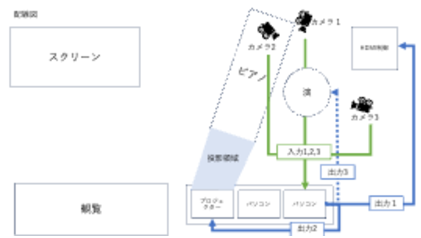
\includegraphics[width=\hsize]{fig/fig3-planet.pdf}
	\caption{プラネタリウムにおける機材の配置}
	\label{fig:planet-system}
\end{figure}


\subsection{演出のねらい}
本作品では，「A Whole New World」の振り返りを踏まえて，より観客の視線を意識した作品制作を行った．具体的には前回の作品では映像がスクリーンのみの投影となり，どうしても観客の視線はそちらに集中されていた．そのため今回は，映像の範囲を拡張することで，空間の中での視線を分散させ，音楽の要素である演奏者や楽器にまで視線が行くようにすることを目標とした．目標達成のために，仕様楽器である，ピアノとに映像を投影し，演奏者を撮影するカメラを複数台置き．映像と合成することにした．

\subsubsection{音楽のテンポによる時間軸表現}
今回筆者が感じた楽曲の切ない様子や目まぐるしく変化する情景をを表現するために使用する楽器をピアノのみとすることにし，演奏者はピアノの経験者とした．今回使用する楽譜はあらかじめ購入したものを使用する\cite{gakuhu}．この楽曲はやや高音部でのイントロから入り，Aメロになると音高が下がり落ち着いた印象となる．しかしサビになると再び音高が挙がるという特徴がある．この対比により，夏の夜の落ち着いた様子と時間が過ぎていく様子が表現されていると考える．間奏部分では八分音符によって音の動きが速く感じられるようになるが，間奏後のCメロ部分のみ全体のBPMより遅くなる．その後97小説目から98小説目にかけて間があいたのちに，もとのBPMに戻ったのと同時に転調してラスサビが始まる．この97小説目から98小説目の間に花火の効果音を入れた．そのことで，ラスサビの盛り上がりに向けた起爆剤的な役割になるのと同時に，夏の夜の静寂さとはかなさを表現する．


\subsubsection{夏の空の映像空間での楽曲表現}
今回作品制作を行う上で，主にAdobeが開発しているモーショングラフィックスとビジュアルエフェクトを行うAfter Effects，ビジュアルプログラミング言語であるMax8の2つのソフトを使用した．

まずAfter Effectsを使用して，スクリーンに投影するための映像と，ピアノに投影するための映像の2つを作成した．スクリーンに投影する映像を動画１とし動画1には演奏者のカメラ映像も投影するため，シーンの切り替えなどをなるべく減らし，演奏者の動きと映像のどちらも引き立たせるような映像にしたいと考え制作した．また，楽曲の過去の恋愛から今に至るまで，時が過ぎていく様子を表現するために夕日の中で雲が流れていく様子や，空がだんだんと暗くなる様子などを表現した．また，2番に入ると，星空の場面になり楽曲のイメージにもある流れ星と時が過ぎていくことを表現するために星が時間ともに動いていく様子を表現した．また，2番の終わりの静寂パートではピアノの演奏に浸ってもらうために，映像をなくした．ラストのサビでは夏の終わりにはかなく終わる恋愛と感情が爆発する様子，また楽曲の美しさを表現するために色とり鳥の花火を打ち上げる様子を取り入れた．これらの映像は1つ1つパラメータを調整し，雲が流れる様子や，流れ星，花火それぞれがリアルに，そして変化を出すようにすることを意識して制作した．ピアノの側面に投影する映像を動画2とし，動画２には歌詞を表示することでより楽曲の世界観に入れるようにし，背景はシンプルな中でも楽曲のイメージを崩さず，またスクリーンと合わせるような工夫をした．

\begin{figure*}[tb]
	\centering
	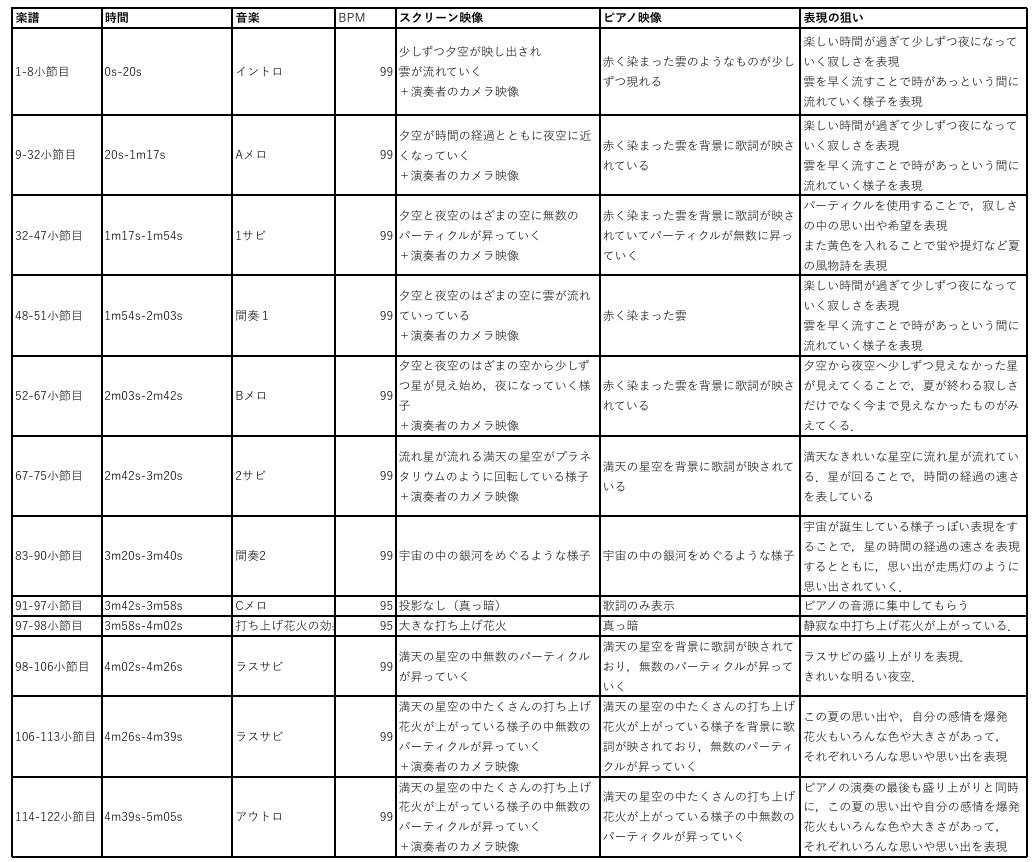
\includegraphics[width=\hsize]{fig/planet.png}
	\caption{プラネタリウムの演出シナリオ}
	\label{fig:planet-scenario}
\end{figure*}

\subsection{システム概要}
次にシステム概要についてまず，求める入出力の関係について\figref{fig:planet-flow}に示す．

\begin{figure}[tb]
	\centering
	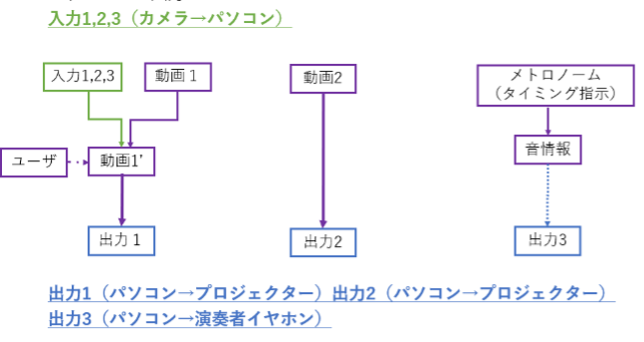
\includegraphics[width=\hsize]{fig/fig4-system.png}
	\caption{システムの入出力の関係}
	\label{fig:planet-flow}
\end{figure}

入力については，iPhone等を用いたWebカメラ3台でリアルタイムで撮影している演奏者の映像をWi-Fiを経由してPCに送信し，入力1，2，3とする．次に出力について，出力1では入力されたカメラ映像と，作成した動画１をMax8内で組み合わせて新たな映像，動画1‘としてHDMIケーブルで天井スクリーンに送信し，スクリーンに投影する．出力2では作成した動画２をHDMIケーブルで用意したプロジェクターに接続し送信する．出力３では演奏者が，映像と合わせてピアノ演奏を行う必要があるため，演奏開始やテンポの指示を出すためのメトロノームを音情報として演奏者のイヤホンにBluetoothで送信する．

Max8では入力されたメラの映像と作成した動画1を合成させる処理を行う．jit.grabというオブジェクトでカメラ映像を受け取り，解像度を指定する．この時の解像度は使用するプロジェクターに合わせて決定した動画の解像度と同じにする必要がある．次にMax8内で認識されているカメラのリストの中から今回使用するカメラ映像を選択する．また，動画1についてもjit.movie~のオブジェクトを使用し．動画1をMax8内で読み込む．それぞれの映像をjit.scissorsを用いてそれぞれを縦横に分割する．それぞれ分割した映像を，jit.glueを用いて合成し，1つの動画を形成する．この時，jit.xfadeを用いて2つのカメラの切り替えが可能になり，これを複数個繋げることで複数のカメラの切り替えが可能となる．ここで生成された映像に全体と動画1の間でjit.xfadeをかけることで，カメラ映像の上に動画1の映像が上乗せされ，画面が完全に分割されたような映像にならず，違和感を減らし，演奏者を引きたてつつも楽曲のイメージの世界観に入り込めるような工夫をした．また，xfadeの値を0\kara 1の間で譜面情報をもとに時系列に沿ってユーザがリアルタイムで変えていくことで，カメラ映像を完全になくすことができるため，動画1の映像の世界観とピアノ演奏に入り込めるような時間を作ることができる．これによって作成した映像を動画1‘としてスクリーンに投影する．以上のシステムで本作品を制作した．

\subsection{作品発表と振り返り}
\subsubsection{作品発表}
本作品を2024年10月7日月曜日に，本学で行われているシニアワークカレッジに参加されている地域の方々10名程度に，同年10月8日火曜日に橋田ゼミのメンバー10名に対し，作品発表を行った．また同年10月29日火曜日に橋田ゼミの1,2,3年生に対して本作品のシステム概要の説明をデモ形式でおこなった．

\begin{figure}[tb]
	\centering
	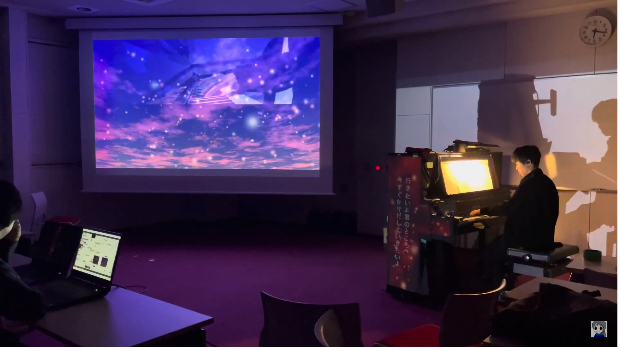
\includegraphics[width=\hsize]{fig/fig5-planet-play.png}
	\caption{プラネタリウムの作品発表}
	\label{fig:planet-play}
\end{figure}


\subsubsection{振り返り}
作品を見た頂いた上記の方々に本作品に関する評価をもらった．多かった評価としてはピアノ側面に歌詞などを投影したことに関すしるポジティブ評価が多数あった．また，曲の展開に合わせて映像が変化していく様子に対しての評価も多数あった，一方で3201教室という空間全体をしっかりとうまく生かしきれてないという意見や，歌詞のフォント，複数画面に対する観客の視線誘導についてもっと工夫するべきだという意見もあった．さらに今回Max8内のシステムで余分な処理が多かったためか，カメラが3台映らずに1台のみしか機能しないといったことがあったため，そのことに対する検証も必要となる．

今後の作品制作に向けて今回はバラード曲を題材とし，楽器はピアノのみを使用したため，次は別のジャンルの楽曲を題材とし，楽器も別の楽器を複数台用いることでまた新たな作品を制作することとする．また次回も今回の発表で使用した3201教室を使用することで，同じ環境でも映像表現によって空間をいかに変えられるかということに重きを置いた作品にしたいと考えている．そのためにも空間全体をうまく使った作品にすること，また演奏者などのその空間にあるものもしっかり活かした作品にすることを目標とした作品制作を行う．


\section{演奏者の魅力を引き出す演出表現}
\subsection{作品制作の背景}
第3回目の作品制作として選んだ楽曲は，YOASOBIの「ラブレター」\cite{loveletter}という楽曲である．この楽曲を選んだ理由として，前回までの2作品はピアノの生演奏に合わせた演出表現を行っていたため，新たな楽器に挑戦したいと考えた．その際に候補として挙がった楽器がトランペットとエレキギターなどであったため，その楽器を活かすことができる楽曲としてこの楽曲を選んだ．また，今回演奏者として協力を依頼した2名は，とても音楽が大好きであり，日常的に演奏等を楽しんでいる．そのような2人自身を象徴する曲としてもふさわしいのではないかと考え，この楽曲を用いた作品制作を行った．

\subsection{ラブレターの世界観}
この楽曲が制作された経緯として，YOASOBIがTOKYO FMの「日本郵便 SUNDAY’S POST」に出演したことをきっかけにスタートした手紙をもとに曲を作る企画「レターソングプロジェクト」\cite{lettersong}というものがあった．リスナーから「ありがとう」をテーマにした手紙を募集し、その中から選ばれた、当時小学6年生の『音楽さんへ』という宛先で、音楽への感謝を綴った1通が原作となって楽曲が制作されたという経緯がある．

4年間音楽に携わるゼミとして活動してきたことや，音楽が大好きな2人の演奏者の魅力を引き出すための題材としてはとてもふさわしい楽曲だと感じ，この楽曲3作品目の作品制作の楽曲として選定した．

\subsection{舞台構成}
本作品も前回の2作品同様3201教室での演出表現を行う．教室の機材配置を\figref{fig:love-system}に示す．
本作品では備え付けのスクリーンを使用せずに，3201教室の壁一面を投影面として映像を投影し，壁前の床にも映像を投影することを目標とする．前回の2作品よりも教室全体を利用した空間演出表現をめざすこととする．プロジェクターは壁に対して3台用意し，床に対して1台用意することとする．また，プラネタリウムの作品と同様に，演奏者に対してそれぞれ1台ずつのカメラを設置することで，演出の一部に組み込んだ．今回もカメラはiPhoneやタブレットを，Webカメラとして使用した．


\begin{figure}[tb]
	\centering
	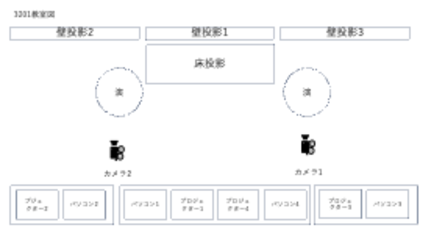
\includegraphics[width=\hsize]{fig/fig6-lovesys.pdf}
	\caption{ラブレターにおける機材の配置}
	\label{fig:love-system}
\end{figure}

\subsection{演出のねらい}
今回映像制作を行うにあたってのコンセプトを複数立てた．まず，1番に表現したいことは「演奏者2人から音楽へのありがとう．音楽から演奏者2人へのありがとう」である．これはこの楽曲が作成された経緯や作品制作でこの楽曲を選定した理由と深く結びついている．そして「音楽によって生み出される自由な世界」「音楽を通した成長など」を作品を通して表現したいと考えた．
\subsubsection{楽器構成における音楽表現}
「ラブレター」という楽曲は，原作の手紙に込められた様々な感謝が，吹奏楽の明るい音楽とともに表現されている楽曲である．今回，使用する楽器をトランペットにあらかじめ決めておいたため，この楽曲とピッタリだと考えた．そこでトランペットを主旋律とした演出表現を行うこととした．しかし，トランペットのみだと音数が少なすぎるため，エレキギターを加えることとした．またこの楽曲では輪唱部分がいくつか存在し，トランペットでその部分も補完する必要があった．しかし，トランペットの演奏者が1人であったため，この楽曲を1人でを完奏することが体力的に難しかった．エレキギターを入れることで，79小説目の最後のラスサビ主旋律をエレキギターとし，輪唱部分をトランペットとすることで，曲の演奏が可能となった．また，最後の転調とともに盛り上がる部分の主旋律の楽器が増えることで，この楽曲の明るさとともに，演奏者，2人の魅力を引き出すことができると考えた．

しかし，まだこの2つの楽器では音数が少なく，ハーモニーやリズム感というものを表現することができなかった．そのため，この2つの楽器のバックにInstrumental音源を流すこととした．
\begin{figure}[tb]
	\centering
	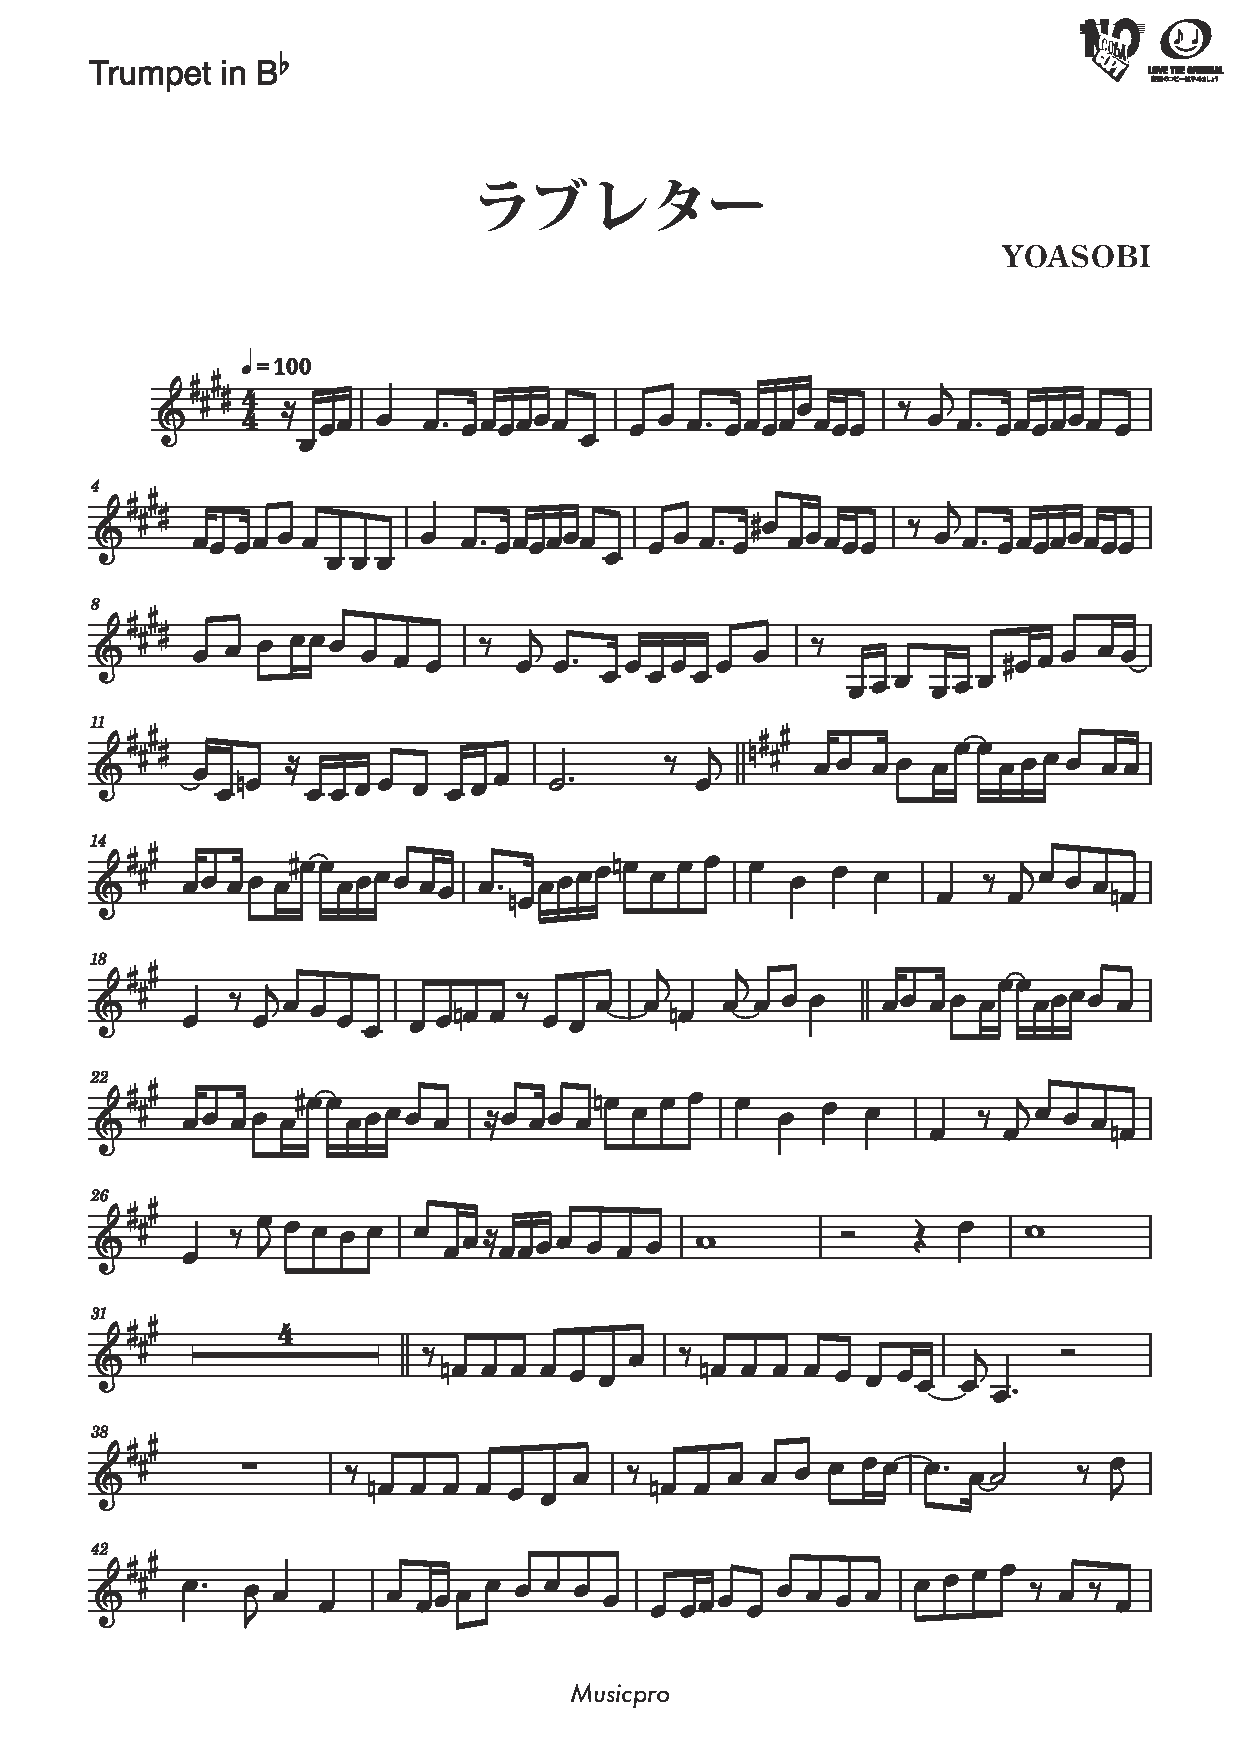
\includegraphics[width=\hsize]{fig/YOASOBI.pdf}
	\caption{「ラブレター」のトランペット用演奏譜}
	\label{fig:YOASOBI}
\end{figure}

\subsubsection{想いを視覚化する映像空間表現}
今回もAfter Effectsを使用した映像生成を行った．また，表現の幅であったり具体的な情景を描写するために複数の生成ＡＩを用いた．さらに，オーディオビジュアルツールのTouchDesignerを用いてリアルタイムでの演出表現を行うこととする．

まず，映像の中心となる正面の投影は，生成AIを用いて演奏者2人が作り出していく世界と，日常の中を音楽を真っ白な本を1ページずつ描いていき1つのストーリとなるようなイメージで制作した．例えば楽曲の最初は2人が，音楽を通じて2人が好きなことなんでも表現できるということを表したかった．そのため，最初は1本の線から始まり，少しずつ彩られていく音楽の世界というものを表現した絵をいれた．その後，日常における音楽というものを，2人の出会いの様子を表現した絵から始まり，季節が過ぎてもそこに存在する音楽というものを生成AIによる絵で再現した．すべてのシーンにおいて2人が用いている楽器が映し出されいるところが特徴だ．間奏に入ると，映像は一面，白くなる．それと同時に3201教室のホワイトボードがある位置に歌詞が表示されるようになり．演奏者2人の音楽への想いを1番表している場面となる．その後，室内の映像が全て暗くなり，歌詞の「受け取ってどうか私の想いを」という文字が表示された後，夕暮れの学校や，街並み．幻想的な湖の風景の中にある楽器たちが映し出される．ここでは演奏者に最も注目してもらいたいため，背景としての役割を持たせている．これと同時に，左右の壁には演奏者2人が演奏している様子が大きく映し出される．この最後の演出以外は左右の壁は，手紙のようなイメージで歌詞が映し出される仕様となっている．最後の2人の演奏者が映し出されるシーンでは，Webカメラを用いてTouchDesignerでリアルタイム制御を行っている．楽曲の最後は再度部屋が全て暗くなり，演奏の音だけが空間に響くようにすることで，聴衆に再度「音楽」というものを感じてもらい余韻に浸ってもらうようにしている．
\begin{figure*}[tb]
	\centering
	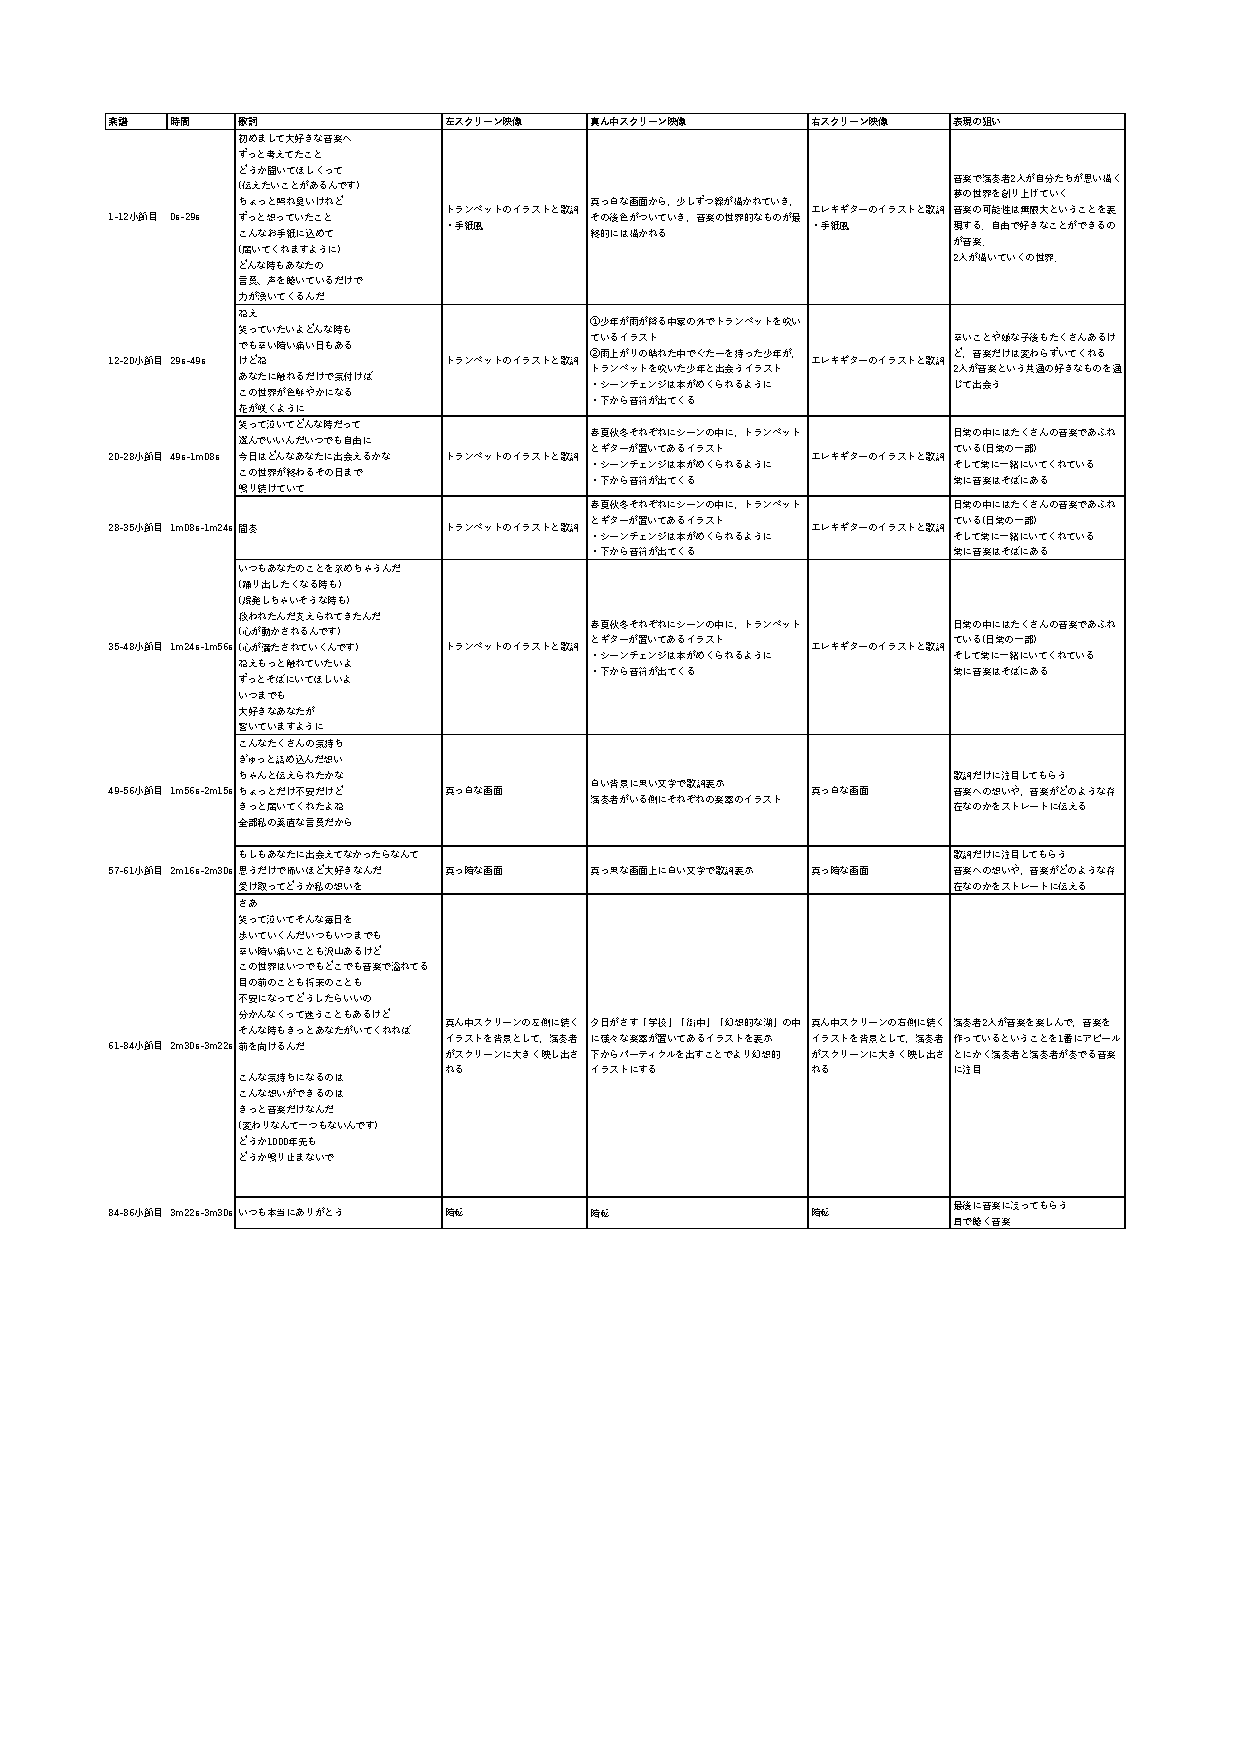
\includegraphics[width=\hsize]{fig/loveletter.pdf}
	\caption{ラブレターの演出シナリオ}
	\label{fig:loveletter}
\end{figure*}

\subsection{作品発表と振り返り}
\subsubsection{作品発表}
現在作品発表に向けて，リハーサルを行っている．最終発表は2月の上旬に行うことを目標に評価と作品の修正を繰り返している．


\begin{figure}[tb]
	\centering
	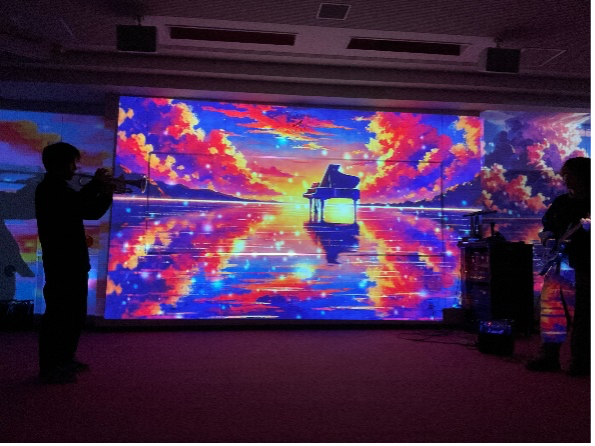
\includegraphics[width=\hsize]{fig/fig7-love-play.png}
	\caption{ラブレターのリハーサル}
	\label{fig:love-play}
\end{figure}



\subsubsection{振り返り}
本作品では，複数台のプロジェクターを用いて壁一面と床への投影を目標として制作を行った．今回プロジェクターの明るさの都合で床への投影がまだできていないが，作品発表に向けて実現できるようにしていきたい．今回，生成AIを使用したことで，表現に幅を持たせることができた．またラスサビの部分で左右の壁に演奏者を大きく映し出すことができ，演奏者の魅力を引き出すことを意識した，ストーリーであったり演出を施すことができた．

一方で空間を活かすという点においてはまだ，壁一面に投影しているという点を活かすことができておらず，迫力に欠ける部分があった．今後，観客の視線誘導なども意識していく必要がある．本作品ではピアノではなく，トランペットとエレキギターを使用しているということを活かし，演奏者の動きや演奏に合わせた演出を加えていきたいと思う．実際に，生演奏における演出表現であるという点をまだ活かしきれていない．そのため作品発表に向けては，空間を活かすことと，な面相であるということを活かすということを意識したうえで作品の修正を行っていきたい．

\section{演出における生成AI}
作品制作にあたって，必要となるものが動画の素材である．本来ならイラストを描いたり，写真や動画等を撮影することでの作品に必要な素材を準備する．しかし，これを1人で実現するにあたっては多くの時間と労力，または美術力等の技術も必要になってくる．そこで前回までの作品制作ではフリー素材から素材を取ってきたり，After Effectsで1から作成した．しかし，やはり自身が望むイラストやシーンを再現することがなかなか難しいことが多かった．そこで，本研究においては生成AIを使用してきた．

今回使用したAIはAdobeExpress\cite{adobeEX}とDALL-Eの2つを主に使用した．AdobeExpressは想像する内容をテキストで記述して画像を生成するものとなっている．一方でDALL-Eもテキストを記述して画像を生成するものとなっている．この2つの大きな違いとして，DALL-Eは対話型の生成AIであるという点がある．これは，演出に使用するための素材を入手する点においては，大きなメリットとなる．対話型生成AIでは，出力された画像に対してもっとこの部分をこのように修正してほしいというような指示をすることができる．一方，テキストをプロンプトするだけのAIでは自身が理想とする出力が得られるまで複数回実行する必要がある．もちろん，どちらのAIも完璧な出力を難しいことは難しいが，細かな設定や情景を少しずつ形を変えながら理想の出力を求めていける点で対話型の生成AIは大きなメリットがある．

また，生成AIで画像を生成する際には文章の入力も気を付ける必要がある．例えば「外が雨の中で少年が部屋の中でトランペットを吹いている風景」という文章がプロンプトされたとする．人間であればこの状況を何となく理解することができるが，AIにとっては，修飾語の関係性が理解されない場合がある，この場合，「雨の中」という文が，「外」のみでなく「少年が」という言葉にも修飾されてしまう場合がある．そのため，句読点を用いてより具体的な状況，この場合は「窓の外で雨が降っている状況で，少年が部屋の中でトランペットを吹いている風景」などと，主語，術後修飾語の関係を明確にする必要がある．


\section{考察}
\subsection{演出における主役}
本研究を通して，最も重要だった点は演出表現において楽曲のどの要素を最も魅せたいのかという点であった．本研究の全ての作品において共通だった点は，演奏者がいて生演奏をすること．そして同じ教室を使用するという点であった．この時点で，魅せる物の要素として「音楽そのもの」「演奏者」「楽器」「教室」などといったものがある．またこれに付随して，音楽の譜面的要素と背景的要素ある．その中で何を観客に魅せたいものなのかによって演出表現の仕方が大きく変わってきたと思う．「A Whole New World」ではアラジンという背景的要素を魅せつつ，初心者におけるピアノ演奏という譜面的要素も考慮する必要があった．「プラネタリウム」では，音楽における時間軸表現といった譜面的要素を表現しながら，作品の制作背景を意識した．さらに最後のラブレターでは演奏を魅せるといった目標のもと作品を制作した．これらの作品制作において演出における主役によって演出手法や表現の仕方などが大きく変わるのだと感じた．

\subsubsection{譜面的要素における演出表現}
譜面的要素を魅せるための演出としては，視覚的な動きや色などにおける表現が重要だったのではないかと考える．譜面的要素は，観客が譜面を直接見たり，まして音楽にあまり知識がない人たちにとっては直感的なものであり，抽象的なものである．そのような要素を視覚的に表現することによって音楽を受け入れやすくなったと感じる．特に映像における動きはテンポと強く結びついており，色は抽象的ながらも感情とリンクさせやすいものである．このように観客にとって直感的な音楽の譜面的要素の表現にはシンプルで分かりやす表現手法が重要であったと考える．

\subsection{背景的要素における演出表現}
一方で背景的要素においては具体的な情報が含まれているため，楽曲における印象はこちらの方で決まりやすい．そのため「A Whole New World」のように作品の世界をそのまま観客に表現するのも1つの手であると考える．一方で，それらを視覚化することで観客に対して楽曲から創造しうる世界や魅力の可能性をつぶしてしまうことにもなりかねない．そのため，楽曲の制作背景を知らなかったり，そもそも楽曲自体を知らない人にとって，演出表現はストーリや独自の世界を創造するヒントや手助けとなる必要がある．背景的要素における具体的な物を視覚化するだけではなく，色や図形など抽象的なものでうまく表現することで，観客自身が音楽の魅力を作るきっかけとなったのえではないかと考える．

\section{おわりに}
本研究では，作品制作を通して空間における音楽映像体験を提供することを目的とした．誰もが再現できるような簡易的な素材と技術を用いて楽器の生演奏に合わせた空間演出を意識して，4年間のゼミ集大成として，本学の3201という同じ空間を使用した作品制作を行った．またその中でも，特に作品制作においては「音楽の譜面的要素」と「音楽の背景的要素」に注目して演出表現を行った．空間内をうまく利用し，映像表現によって視覚表現を付与することで，観客に対して楽曲の世界観に引き込み，楽曲の素晴らしさやそこから感じて自らが楽曲の世界を想像することに対する可能性を広げるための空間政策の追及をできたのではないかと思う．






\begin{acknowledgment}
	%本稿の執筆にあたり，参考文献に挙げた方々のWebサイト，スライド，各種資料を大いに参考にさせていただいた．
	書くならお好きに
\end{acknowledgment}

% ---------------------------------------------
% 参考文献 へつづく（imazato-home.texへ)